\input{configuration}

\title{Lecture 1 --- Database Systems}

\author{Jeff Zarnett \\ \small \texttt{jzarnett@uwaterloo.ca}}
\institute{Department of Electrical and Computer Engineering \\
  University of Waterloo}
\date{\today}


\begin{document}

\begin{frame}
  \titlepage

 \end{frame}

\begin{frame}
\frametitle{Course Syllabus}

As our first order of business, let's go over the course syllabus.

\end{frame}

\begin{frame}
\frametitle{Collaborative Course}

The source material for the ECE~356 notes and slides is open-sourced via Github. 

If you find an error in the notes/slides, or have an improvement, go to \url{https://github.com/jzarnett/ece356} and open an issue. 

If you know how to use \texttt{git} and \LaTeX, then you can go to the URL and submit a pull request (changes) for me to look at and incorporate!


\end{frame}


\begin{frame}
\frametitle{Databases}

\begin{center}
	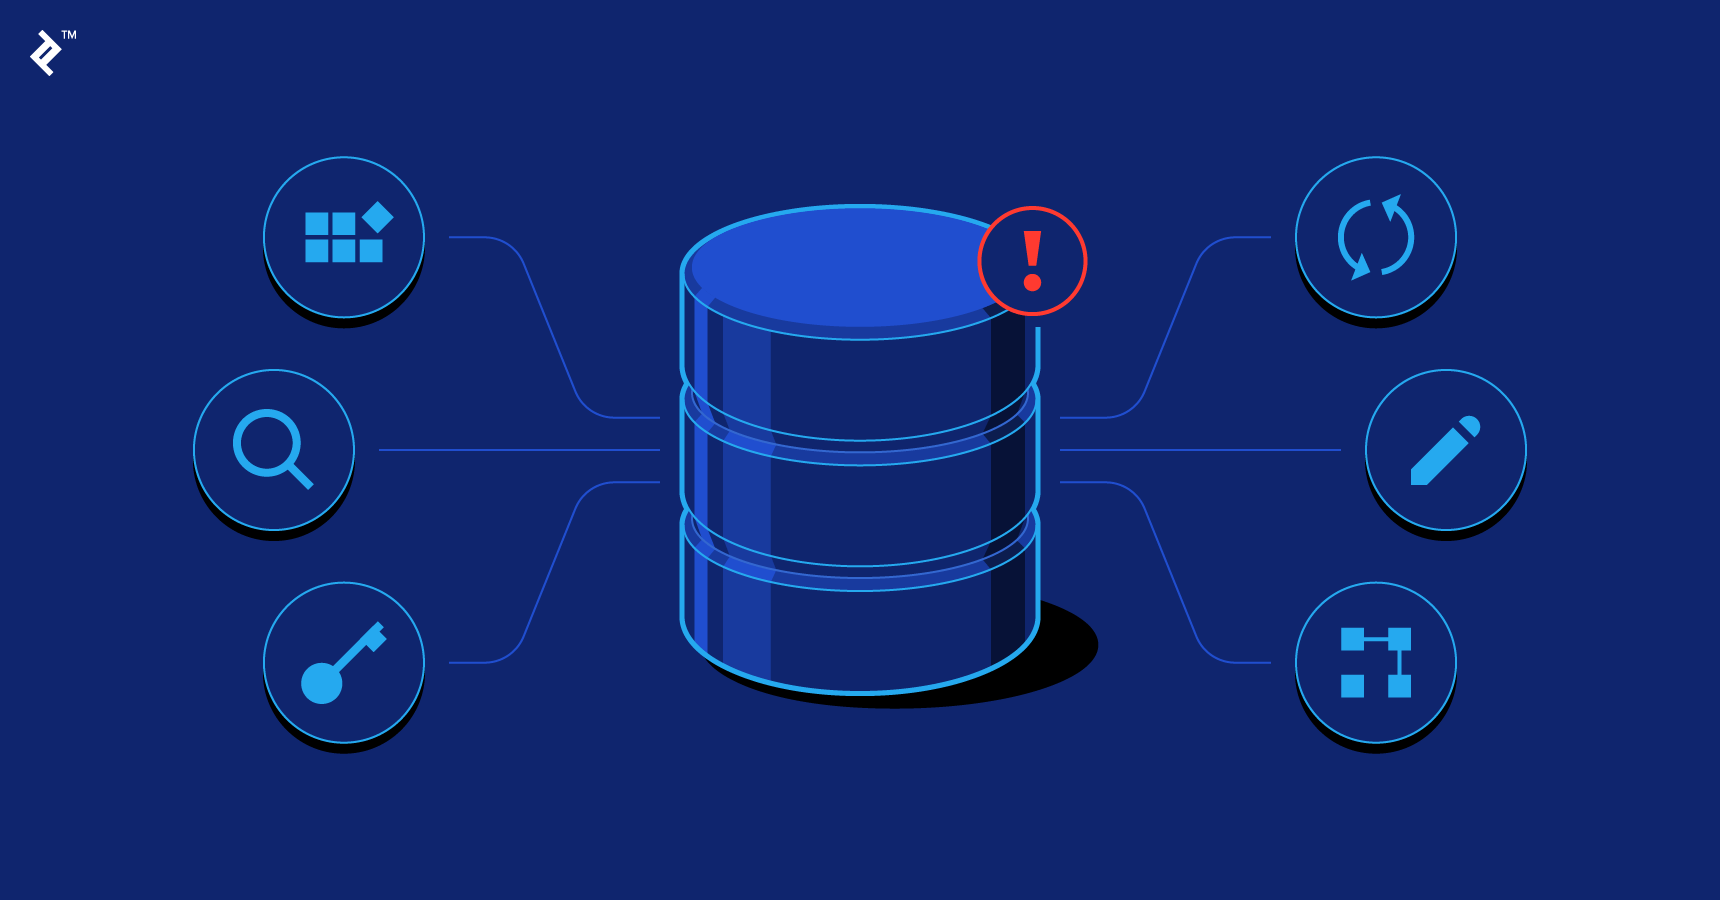
\includegraphics[width=\textwidth]{images/database-img.png}
\end{center}


\end{frame}


\begin{frame}
\frametitle{Databases}

Databases and database systems are everywhere. 

It is safe to say that it would not be possible for you to read this pdf (or attend the lecture in which it is used) without the involvement of databases.

They store data in an orderly fashion and allow for its retrieval at a later date.

The more traditional examples relate to everyday life for a common person: banking, airline reservations, e-commerce websites...

\end{frame}



\begin{frame}
\frametitle{Database ``Alternatives''}
A database is by no means the only way to store data -- any format works.


\begin{center}
	
\includegraphics[width=0.4\textwidth]{images/excel.jpg}
\end{center}

This is not because of the mathematical functions or intelligence of Excel but rather the gridlines. Seriously.

\end{frame}



\begin{frame}
\frametitle{Structure}

For small amounts of data it may not matter very much that the data is not structured and not organized. 

For larger amounts of data, this quickly becomes impractical. 

Some sort of structure is needed. 

\end{frame}

\begin{frame}
\frametitle{First Approach}

First approach: use files.

\begin{center}
	
\includegraphics[width=0.5\textwidth]{images/ducttape.jpg}
\end{center}

\end{frame}


\begin{frame}
\frametitle{Why Not Files?}
\begin{itemize}
	\item \textbf{Data Redundancy}
	\item \textbf{Data Inconsistency}
	\item \textbf{Data Isolation}
	\item \textbf{Integrity Problems}
	\item \textbf{Atomicity Problems}
	\item \textbf{Concurrent-Access Problems}
	\item \textbf{Security Problems}
\end{itemize}
\end{frame}



\begin{frame}
\frametitle{The DBMS}

A database management system (DBMS) is a solution to these problems. 

Of course, a database, if poorly designed, will not fix all of those problems. 

\end{frame}



\begin{frame}
\frametitle{The DBMS}

There are three levels of abstraction we are interested in when discussing a database, from least abstraction to most:

\begin{enumerate}
	\item Physical Level
	\item Logical Level
	\item View Level
\end{enumerate}

\end{frame}



\begin{frame}
\frametitle{Tip Your Server}

A database is typically accessed via a database server. 

\begin{center}
	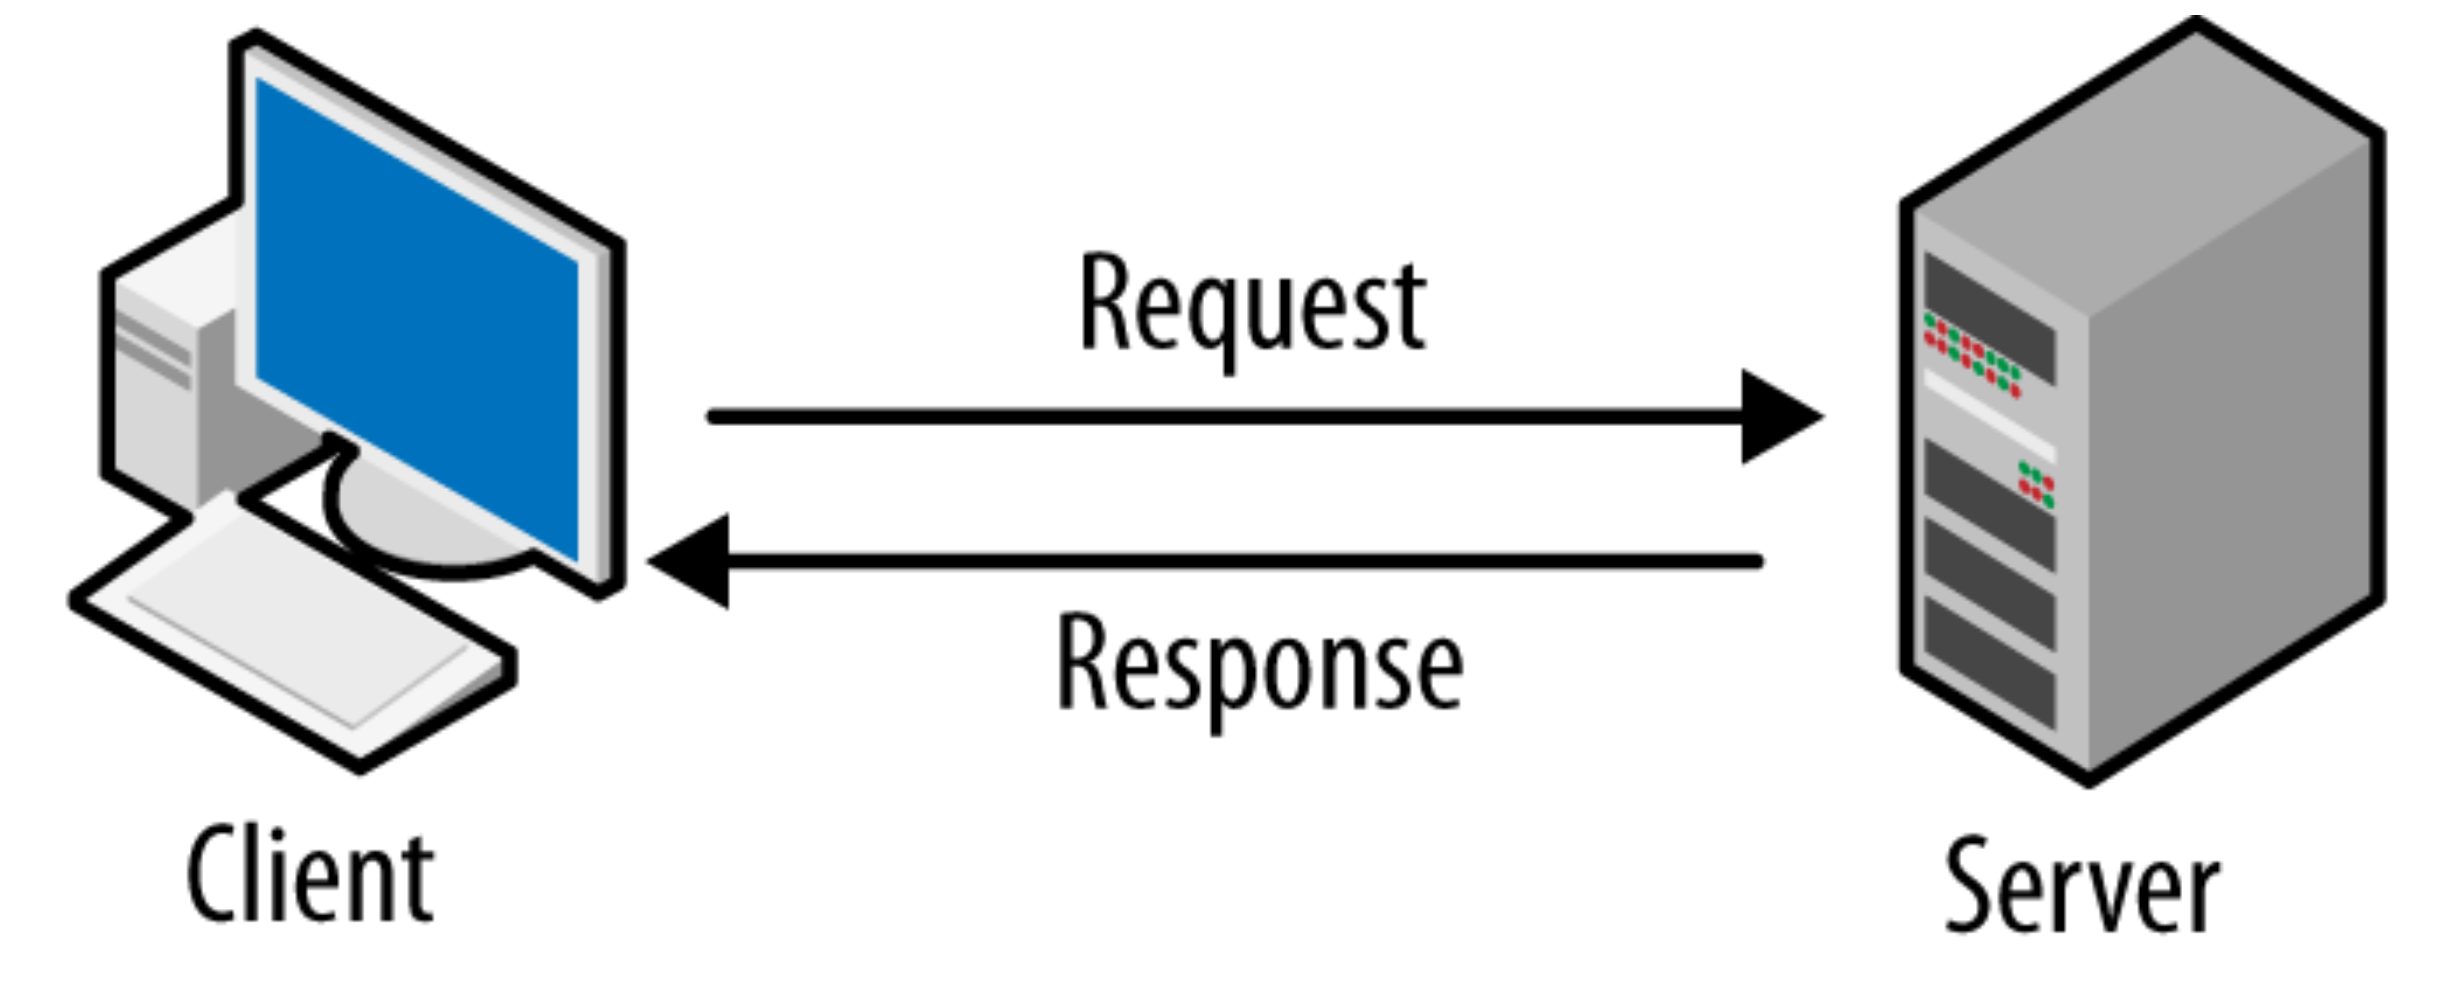
\includegraphics[width=0.6\textwidth]{images/client-server.png}
\end{center}

Thus we see the client-server model in use: an application program then accesses the database through some request interface and receives answers. 

\end{frame}



\begin{frame}
\frametitle{Tip Your Server}

We can also issue statements that change the data directly.

An incorrect statement can do a lot of damage and lead, perhaps, to unrecoverable data loss. 

\begin{center}
	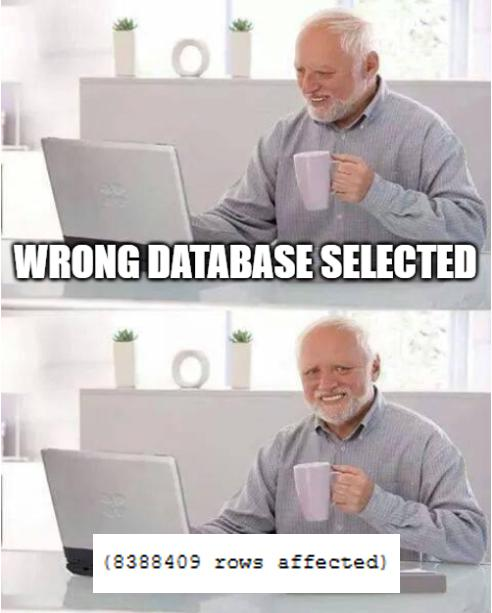
\includegraphics[width=0.3\textwidth]{images/wrong-db.jpg}
\end{center}

\end{frame}



\begin{frame}
\frametitle{Schemas \& Instances}

A database \alert{schema} defines the structure of the database. 

This includes what data is  to be stored in what format. 

An instance of a database reflects both the schema and the particular content of that database.

\end{frame}



\begin{frame}
\frametitle{Sample Logical Schema}


	\textbf{VEHICLE}\\
	\begin{tabular}{|l|l|}\hline
		\textbf{VIN} & \texttt{string(17) not null, primary key}\\ \hline		
		\textbf{year} & \texttt{integer not null}\\ \hline
		\textbf{make} & \texttt{string(64) not null}\\ \hline
		\textbf{model} & \texttt{string(64) not null}\\ \hline		
		\textbf{license\_plate\_number} & \texttt{string(8)}\\ \hline		
	\end{tabular}
	
	\textbf{LICENSE\_PLATE}\\
	\begin{tabular}{|l|l|}\hline
		\textbf{number} & \texttt{string(8) not null, primary key}\\ \hline
		\textbf{expiry} & \texttt{date} \\ \hline
		\textbf{owner\_address\_id} & \texttt{integer}\\ \hline		
	\end{tabular}
	
		\textbf{OWNER\_ADDRESS}\\
	\begin{tabular}{|l|l|}\hline
		\textbf{id} & \texttt{integer not null,  primary key}\\ \hline
		\textbf{name} & \texttt{string(64) not null}\\ \hline
		\textbf{street} & \texttt{string(64) not null}\\ \hline
		\textbf{city} & \texttt{string(32) not null}\\ \hline
		\textbf{province} & \texttt{string(2) not null}\\ \hline
		\textbf{postal\_code} & \texttt{string(7) not null}\\ \hline

	\end{tabular}

\end{frame}



\begin{frame}
\frametitle{Meta-Data in a Schema}

There are also some items of meta-data (data about data) in the shown schema.

\texttt{id} is shown as ``primary key'', which provides additional information and additional restrictions.

There are also indexes that are used in searches. 

They can be added, removed, modified without affecting the underlying data.


\end{frame}



\begin{frame}
\frametitle{Physical Schema}

No information is shown here about how the physical schema looks. 

How is this data stored in a practical sense? 

From the logical view it is irrelevant.

\end{frame}



\begin{frame}
\frametitle{Creating an Instance}

If we create a new database and apply this schema, we created a new instance but it is empty. 

This is the initial state of the database and each modification to the database creates a new state of the database.

At any time, we can take a snapshot of the current database (export all its data). 

\end{frame}



\begin{frame}
\frametitle{Making Changes}

The most common type of modification would be to manipulate data in it.\\
\quad Add, modify, delete...

This kind of change does not modify the schema, but it does modify the data.

\end{frame}



\begin{frame}
\frametitle{Making Changes}

If we attempt to modify the data in a way that is not consistent with the schema (e.g., try to put ``ABC'' in an integer field), that modification will be rejected.

An update can overwrite or permanently delete important data!

\end{frame}



\begin{frame}
\frametitle{Schema Design}

Careful schema design, as we will see, will prevent that sort of error, such as introducing a requirement that VINs be unique. 

If that rule exists, the update is rejected. 


\end{frame}



\begin{frame}
\frametitle{Schema Design}

Design cannot prevent all such errors, unfortunately. 

There can be two people with the name ``Thomas Anderson''\footnote{Whoah.}, so no rule of unique names can be introduced.

An erroneous update command could set all names to exactly that even if the schema is designed perfectly.


\end{frame}




\begin{frame}
\frametitle{Schema Changes}

Textbook authors sometimes tell you that schema changes will be rare, but much depends on your application. 

\begin{center}
	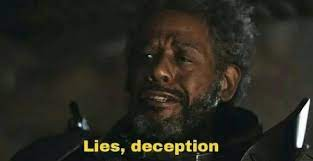
\includegraphics[width=0.5\textwidth]{images/lies.jpg}
\end{center}

If it is a startup company or an app with ever-expanding functionality then the the schema will change regularly. 

Schema changes are design changes.

\end{frame}



\begin{frame}
\frametitle{Schema Changes}

Modifications to the schema can be made in a way that does not affect the data or require changes to applications that access it. 

If a new field ``country'' is added to the address entity, then something that looks only for the name will not be affected. 

Similarly, a new entity, unrelated to these, such as ``Service Ontario locations'' can be created with no impact on the existing data.

\end{frame}



\begin{frame}
\frametitle{Changer Danger}

Modifying a schema, can, of course, be dangerous. 

If we decide to remove a data element, such as the province from the address, then data may be lost. 

If we add another property, such as a country, by default it contains nothing. 

If this property is to be defined as ``not null'' then a default value is needed.


\end{frame}



\begin{frame}
\frametitle{Multiple Instances and Schemas}

The database server can, of course, have multiple instances, and multiple schemas, all of which are independent of one another. 

Two databases may use the same schema but have completely different data.

Two databases can begin with the same schema but evolve in different directions over time based on the changes that are made. 

A change in the schema may result in changes to some data, but may not.

\end{frame}



\begin{frame}
\frametitle{Relationship Goals}

The entities themselves are only a part of the picture.

There are also the relationships between these, which are partially reflected in the fields like \texttt{owner\_address\_id}. 

This takes us to our next subject, which is to examine the relational model.

\end{frame}





\end{document}

